\chapter{Results and Discussion}\label{ch:evaluation}
\section{Training progress and early stopping}
Figure~\ref{fig:learning} summarizes the recorded validation history. The four distant goals remain fixed, whereas the six stage-validation goals become harder after curriculum promotion. Success on the fixed distant set becomes consistent after approximately 560,000 transitions. Both sets pass at 650,000, 660,000 and 670,000 transitions, triggering the configured early stop. The final policy has 670,000 recorded transitions even though the requested ceiling was two million.

\begin{figure}[htbp]\centering
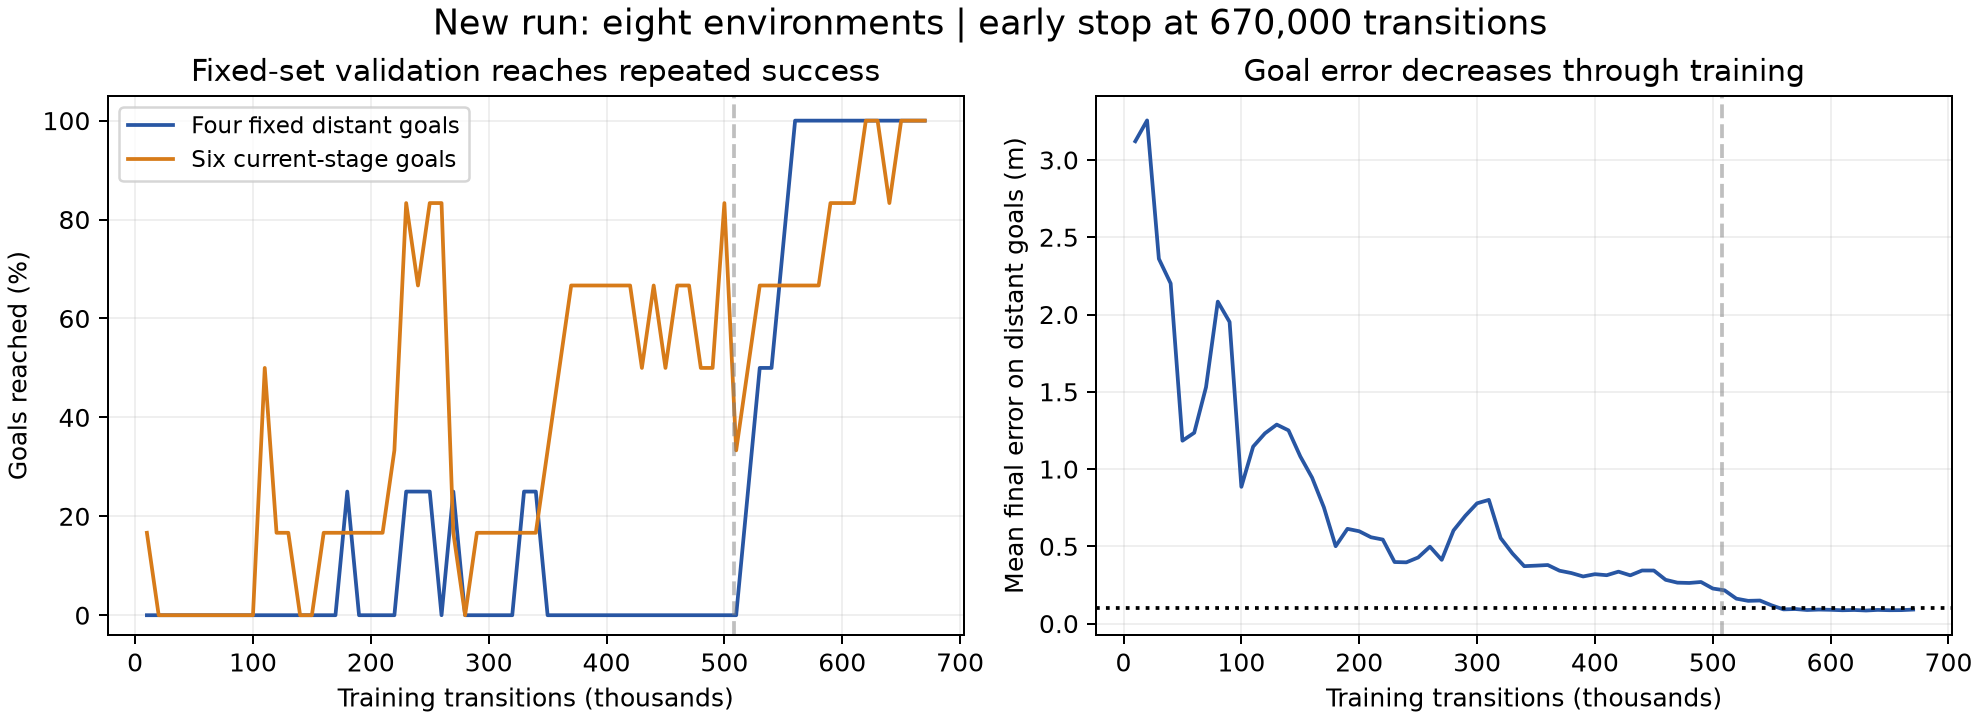
\includegraphics[width=\textwidth]{learning_progress.png}
\caption{Validation history for the reported eight-environment run. The dashed vertical line marks 507,904 transitions, the end of the earlier same-seed run. Current-stage goals change on curriculum promotion. The repeated end-of-training validation is counted only once in this plot.}\label{fig:learning}
\end{figure}

The run contains 1,639 completed training episodes: 655 goals, 917 timeouts and 67 out-of-bounds terminations. These totals include early unsuccessful learning. In the final hundred episodes, ninety succeed. After the full goal distribution is enabled, 336 of 461 completed episodes succeed and no out-of-bounds termination is recorded. These observations indicate improvement during learning, but do not independently certify the final deterministic policy.

The selected checkpoint at 630,000 transitions passes the four distant goals and all six stage goals. The final model also passes both sets. They differ because selection uses a lexicographic validation score, not simply the most recent training step. Both are retained and evaluated to make this distinction explicit.

\section{Additional goal-reaching tests}
Table~\ref{tab:goals} and Figure~\ref{fig:goals} report the sixty-goal evaluation. Both checkpoints achieve 59/60 successes, or 98.3\% observed success. This is a count on the specified evaluation set, not an estimated universal success probability. The obstacle is distant in these trials, so the measurement concerns navigation without active obstacle avoidance.

\begin{table}[htbp]\centering
\caption{Additional goal tests; twenty goals per distance group.}\label{tab:goals}
\begin{tabular}{lrrrr}\toprule
& \multicolumn{2}{c}{Validated 630k} & \multicolumn{2}{c}{Final 670k}\\
Group & Success & Mean error (m) & Success & Mean error (m)\\\midrule
Near & 20/20 & 0.0815 & 20/20 & 0.0795\\
Medium & 20/20 & 0.0812 & 20/20 & 0.0675\\
Distant & 19/20 & 0.0834 & 19/20 & 0.0851\\\bottomrule
\end{tabular}\end{table}
\begin{figure}[htbp]\centering
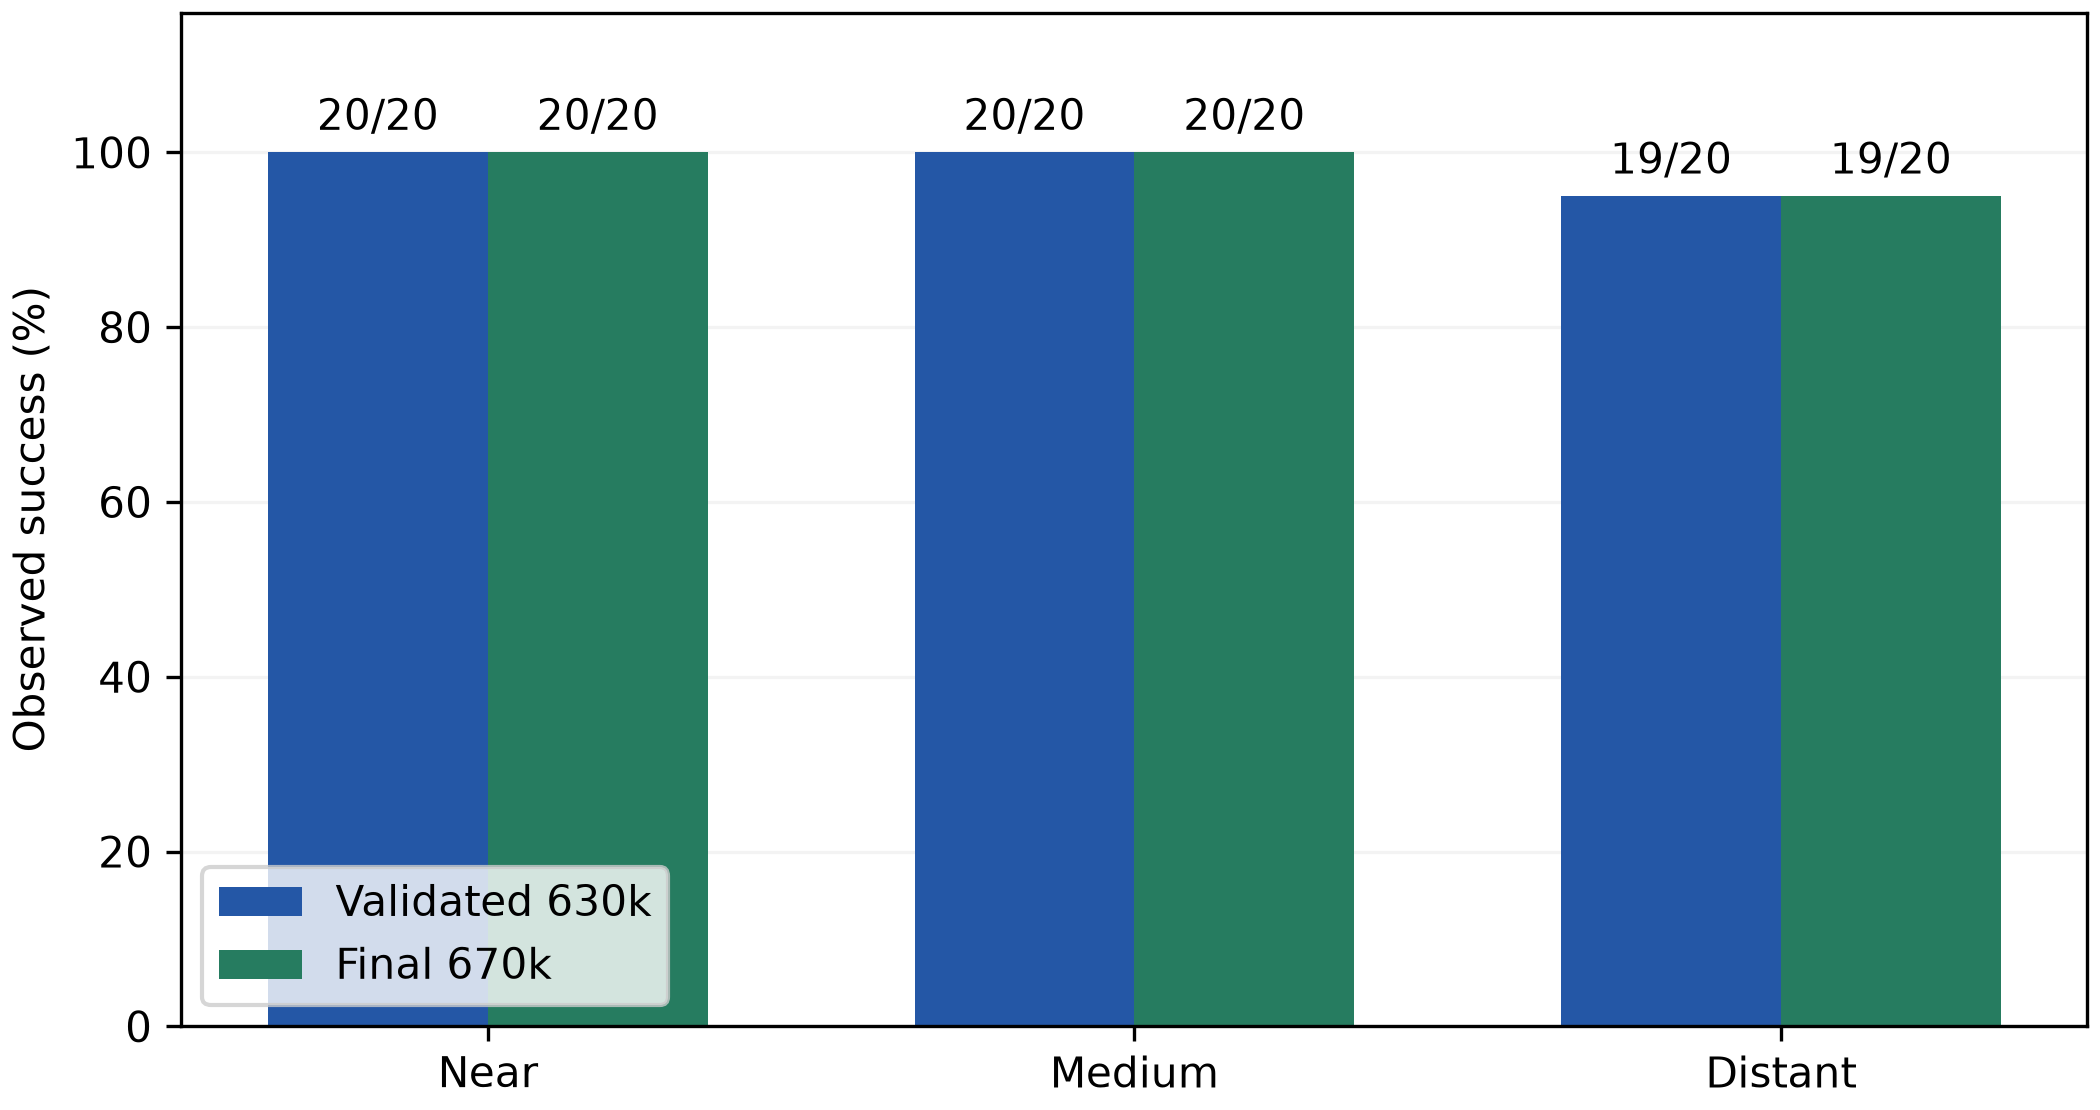
\includegraphics[width=.80\textwidth]{goal_generalization.png}
\caption{Observed success on the same additional goal set for the two checkpoints. No out-of-bounds event occurred in these tests.}\label{fig:goals}
\end{figure}

Both policies fail the same target, approximately $[0.9412,-4.7667,2.9977]^\mathsf{T}$~m. The selected checkpoint finishes 0.1097~m away and the final checkpoint 0.1344~m away. Their closest distances are 0.1021 and 0.1034~m, respectively: neither enters the original 0.10~m acceptance radius. Their final speeds are small, indicating a residual position offset rather than a high-speed pass through the target. The tolerance is not relaxed to convert this failure into a success.

The final model averages 6.42~s over the sixty episodes, including the timeout, compared with 7.20~s for the selected model. This aggregate mixes short and long tasks and should not be interpreted as the time required for the separate five-metre scenario mission. It also shows that the selected and final models are not uniformly ordered on every metric.

\section{Scenario results for the selected model}
Table~\ref{tab:selected} uses only the automatically selected 630,000-step checkpoint. All nine controller/scenario combinations reach the shared goal. The nominal PPO is identical between pure RL and RL+ACBF. Figure~\ref{fig:comparison} summarizes arrival and separation, and Figure~\ref{fig:goalerrors} shows the goal-error histories.

\begin{table}[htbp]\centering\small
\caption{Main scenario results for the validated checkpoint. $d_{\min}$ is centre separation, not surface clearance. Cases 1--3 are linear, accelerating and figure-eight motion.}\label{tab:selected}
\begin{tabular}{llrrrr}
\toprule
Case & Controller & Time (s) & Error (m) & $d_{\min}$ (m) & Path (m)\\
\midrule
1 & Pure RL & 13.70 & 0.089 & 2.067 & 7.628 \\
1 & RL+ACBF & 13.70 & 0.089 & 2.067 & 7.628 \\
1 & PID+ACBF & 7.60 & 0.086 & 1.828 & 5.087 \\
\addlinespace
2 & Pure RL & 13.70 & 0.089 & 1.072 & 7.628 \\
2 & RL+ACBF & 13.80 & 0.088 & 1.211 & 7.386 \\
2 & PID+ACBF & 7.85 & 0.087 & 1.003 & 5.095 \\
\addlinespace
3 & Pure RL & 13.70 & 0.089 & 0.464 & 7.628 \\
3 & RL+ACBF & 13.60 & 0.078 & 0.770 & 7.441 \\
3 & PID+ACBF & 7.80 & 0.085 & 0.842 & 5.099 \\
\bottomrule
\end{tabular}
\end{table}
\begin{figure}[htbp]\centering
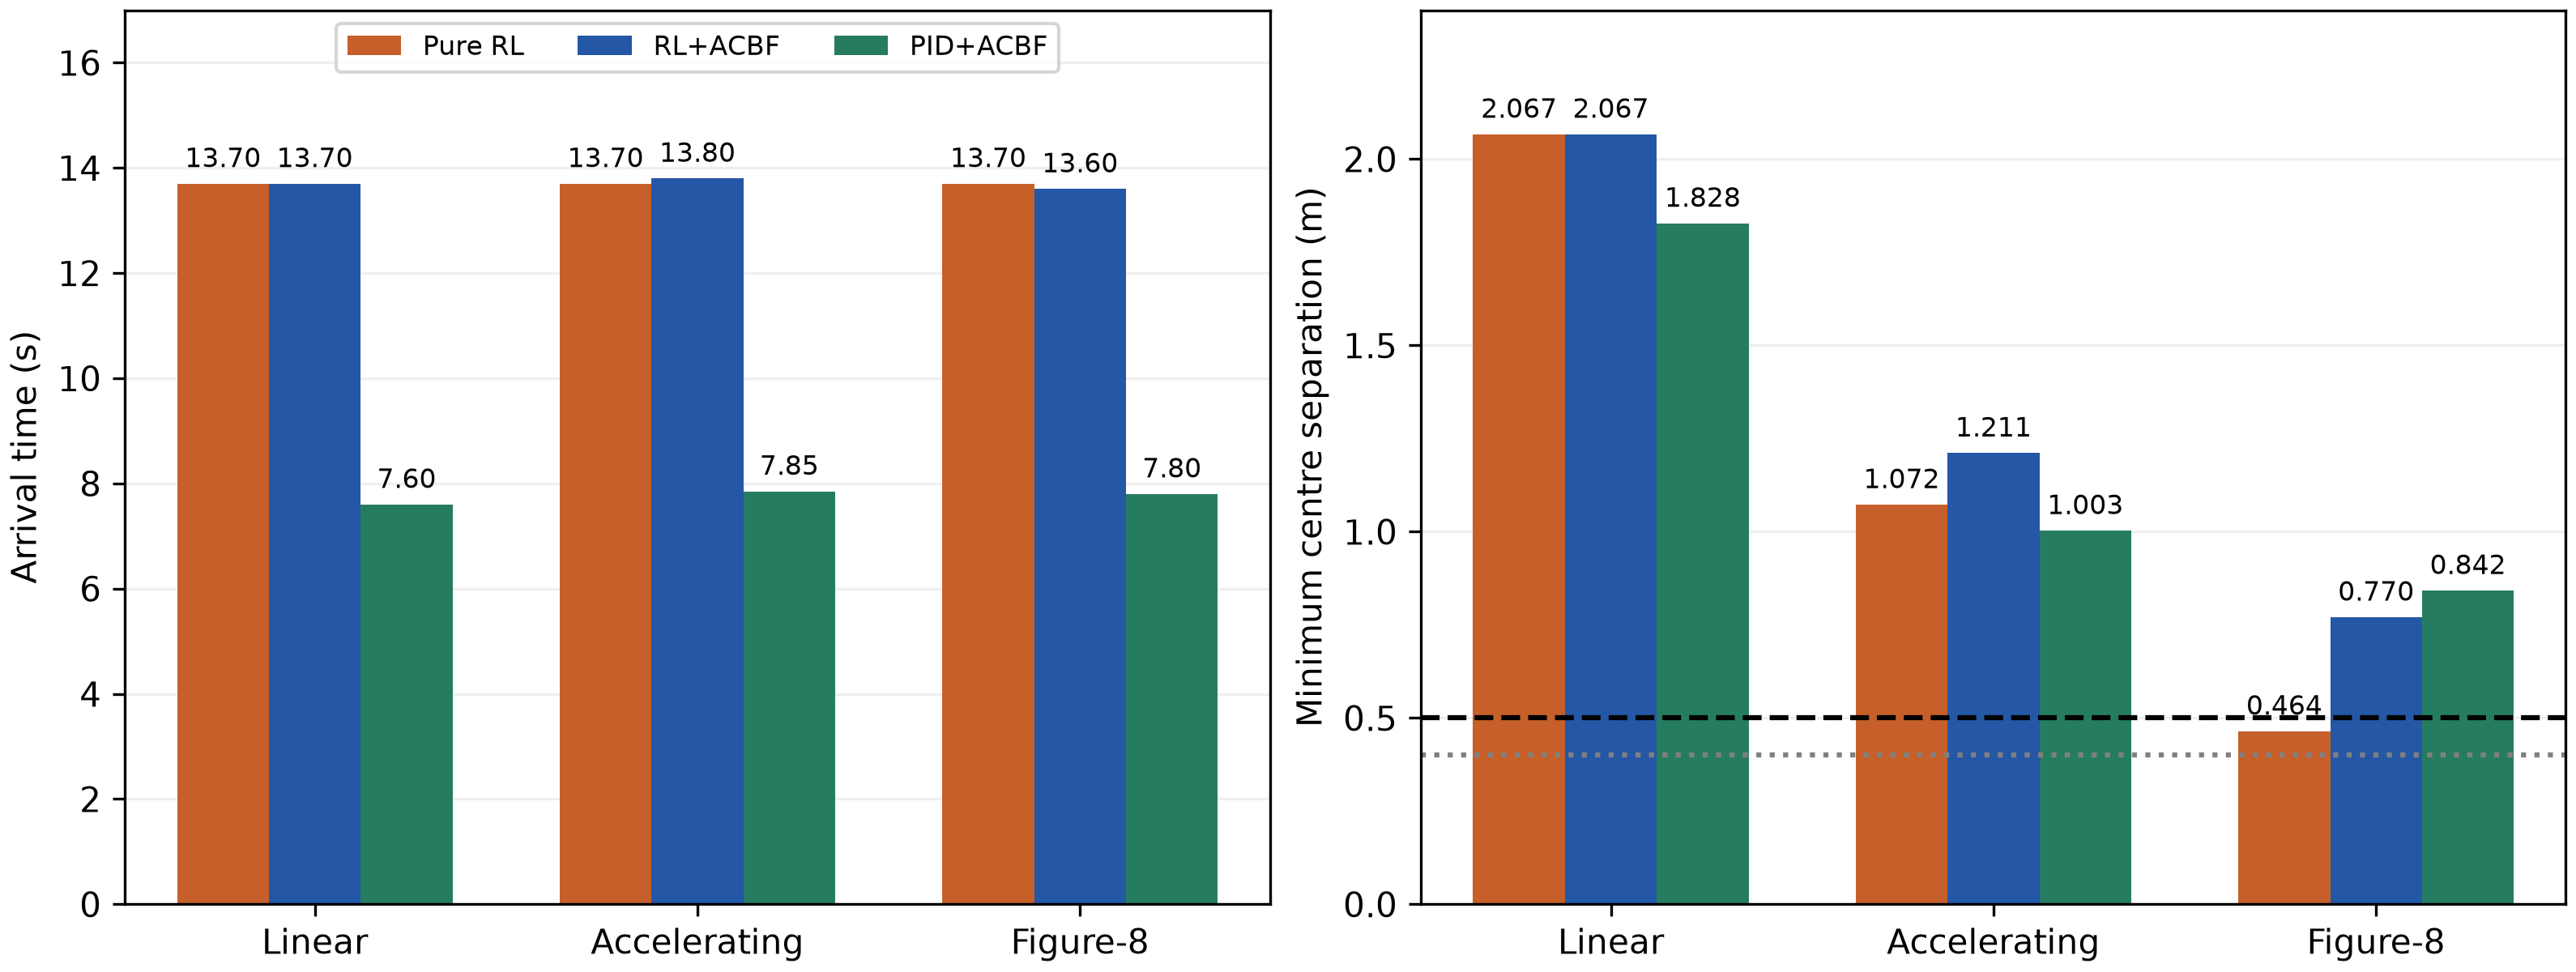
\includegraphics[width=\textwidth]{selected_comparison.png}
\caption{Selected-checkpoint comparison. In the right panel the dashed line is the 0.50~m safety boundary and the dotted line is the 0.40~m collision threshold.}\label{fig:comparison}
\end{figure}
\begin{figure}[htbp]\centering
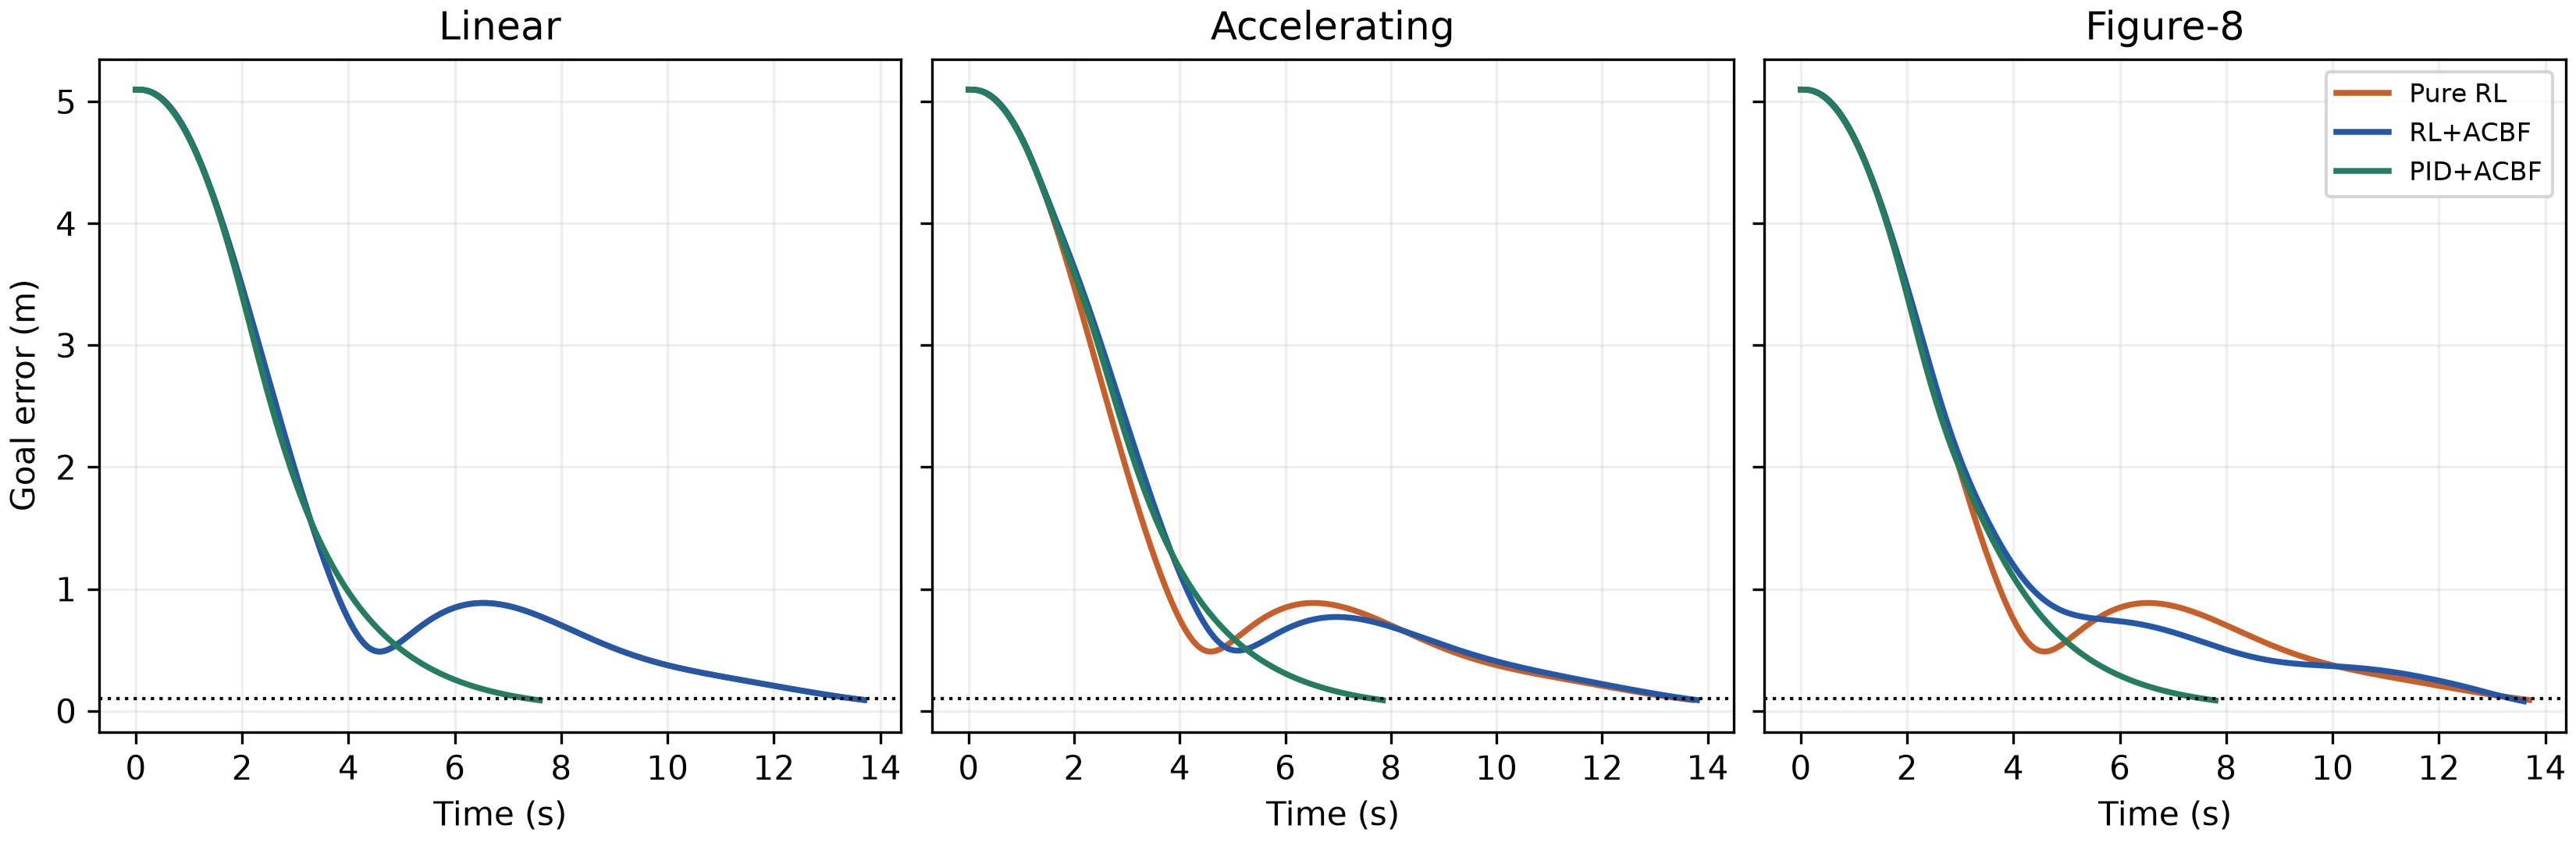
\includegraphics[width=\textwidth]{selected_goal_errors.png}
\caption{Goal-error histories for the selected checkpoint. The dotted horizontal line is the 0.10~m position tolerance; arrival additionally requires the speed and hold-time conditions.}\label{fig:goalerrors}
\end{figure}

\subsection{Linear obstacle}
In case 1, pure RL and RL+ACBF have the same trajectory and arrive in 13.70~s. Their minimum centre distance is 2.067~m, comfortably above the buffer boundary. The nominal trajectory does not require alteration by the filter in this case. PID+ACBF reaches the goal in 7.60~s with a shorter path. Thus the filter's pass-through behavior can be observed without implying an efficiency advantage for RL.

\begin{figure}[htbp]\centering
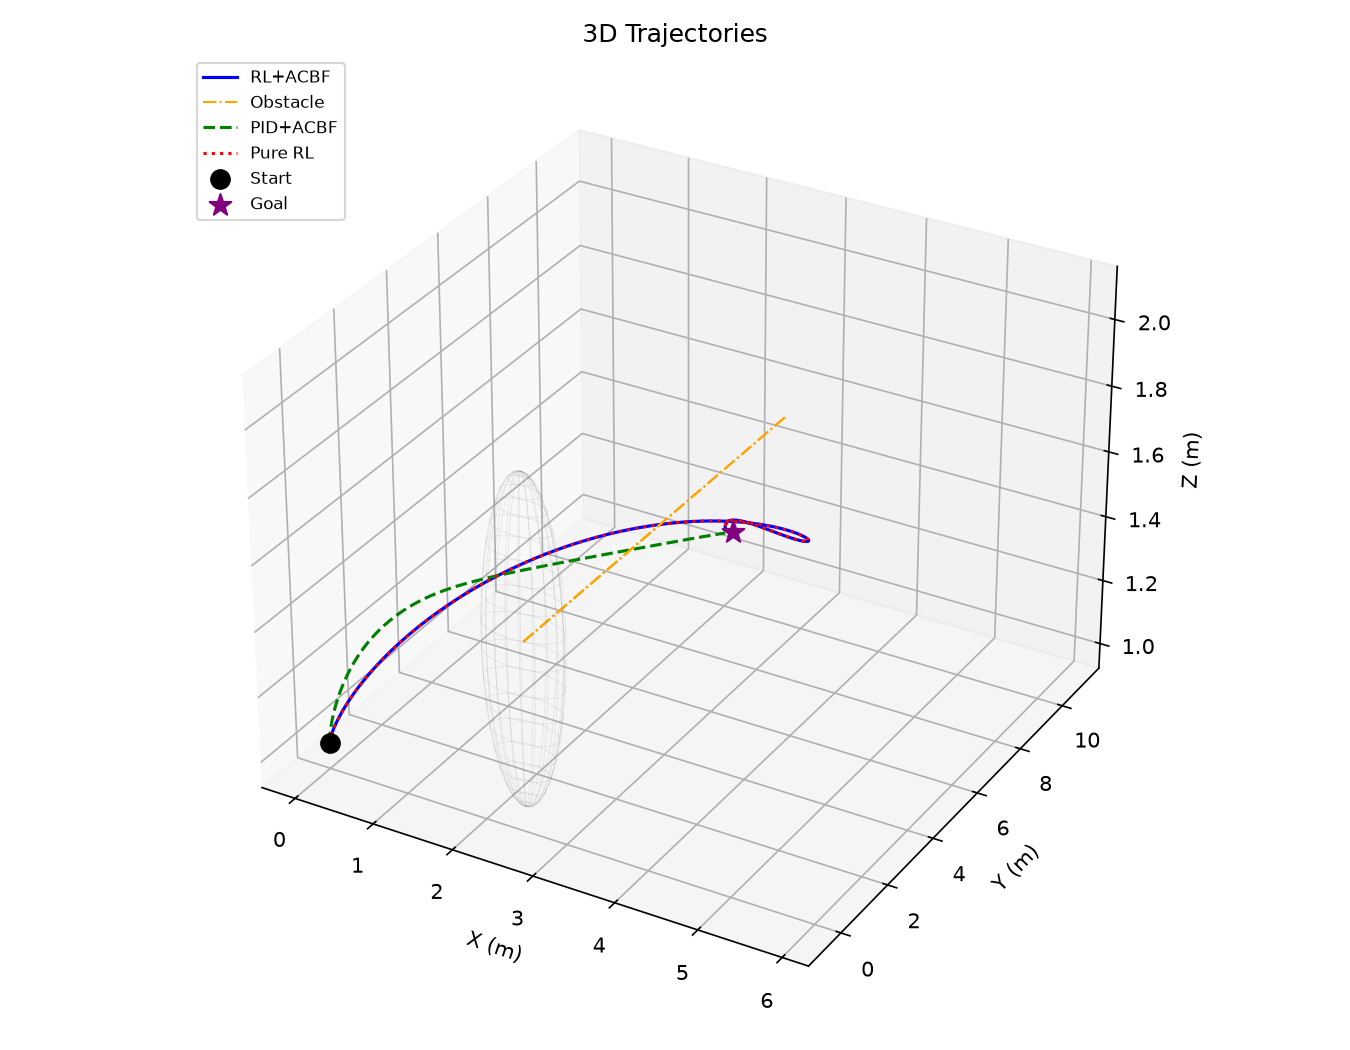
\includegraphics[width=.72\textwidth]{case1_trajectory.png}
\caption{Case 1 trajectories for the selected checkpoint. A spatial trajectory plot does not by itself establish time-aligned obstacle clearance; that is measured from the logged states.}\label{fig:case1}
\end{figure}

\subsection{Accelerating obstacle}
In case 2, the obstacle accelerates across the nominal flight region. Adding ACBF increases minimum centre separation from 1.072 to 1.211~m. Arrival changes from 13.70 to 13.80~s, while sampled path length decreases from 7.628 to 7.386~m. A filter-induced change in state can affect the later policy trajectory, so a larger safety distance does not necessarily imply a longer path. These are measured outcomes for this case, not a general optimality statement.

\begin{figure}[htbp]\centering
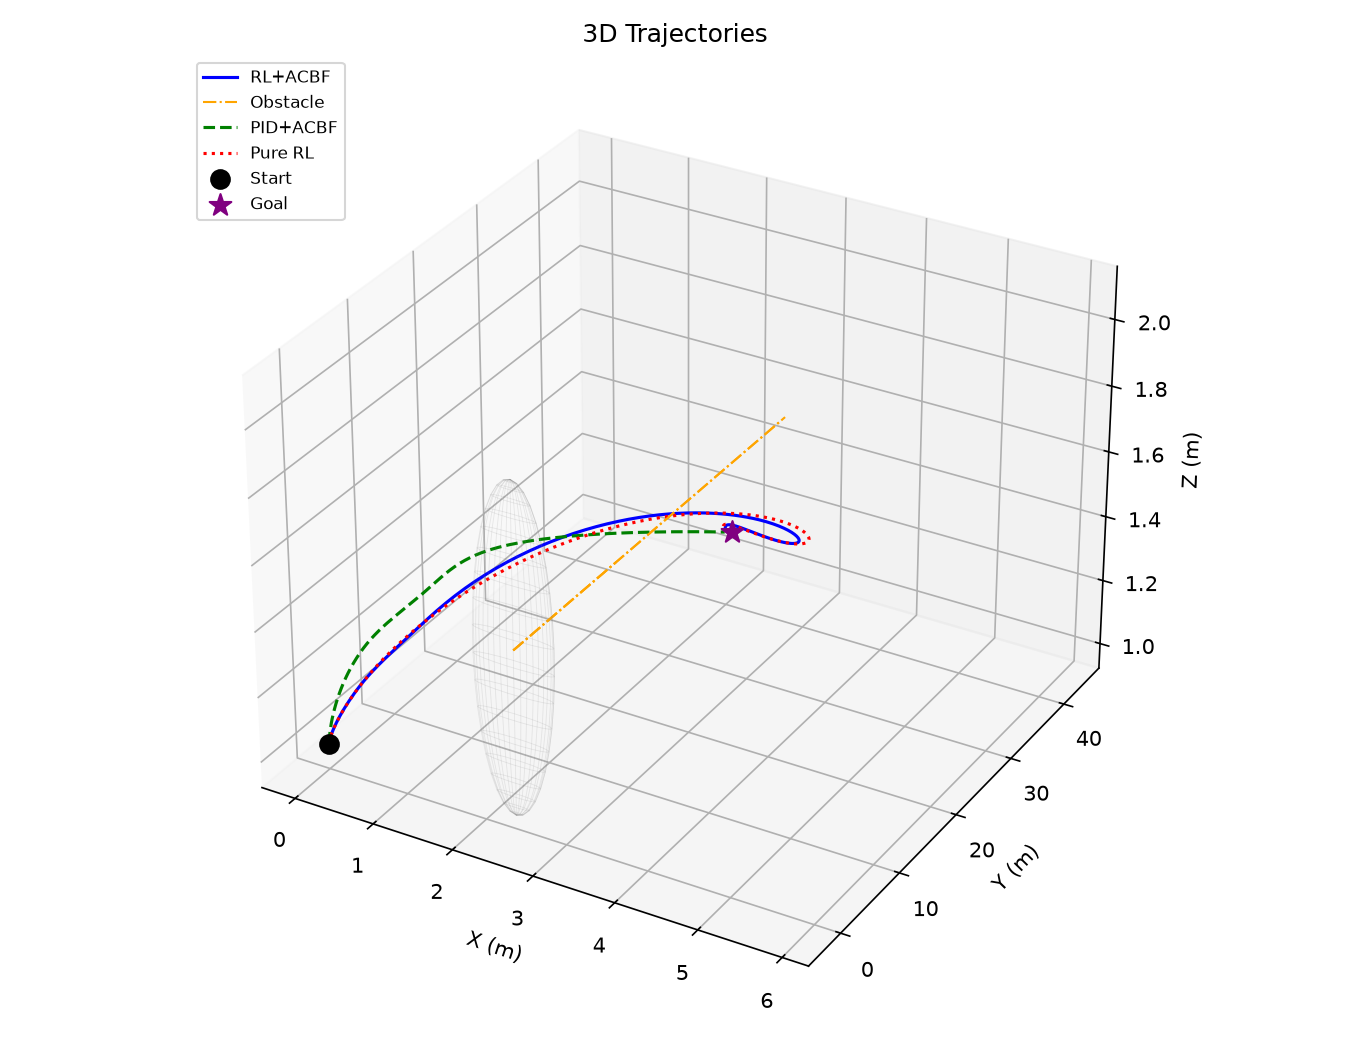
\includegraphics[width=.72\textwidth]{case2_trajectory.png}
\caption{Case 2 trajectories for the selected checkpoint. Both RL variants arrive, while the filtered path maintains a larger sampled minimum separation.}\label{fig:case2}
\end{figure}

\subsection{Figure-eight obstacle}
Case 3 is the clearest demonstration of the filter's measured safety-buffer benefit. Pure RL reaches the goal but attains a minimum centre distance of 0.464~m. This is below the 0.50~m safety boundary and above the 0.40~m geometric collision threshold. It is a buffer violation, not a recorded collision.

RL+ACBF maintains a minimum centre distance of 0.770~m and reaches the goal in 13.60~s. The increase in minimum separation is approximately 0.306~m. Surface clearance changes from 0.064 to 0.370~m. The filtered trajectory also arrives 0.10~s earlier than pure RL. This small time difference should not be interpreted as a reliable speed advantage across tasks, but it shows that preserving the observed buffer need not prevent arrival.

\begin{figure}[htbp]\centering
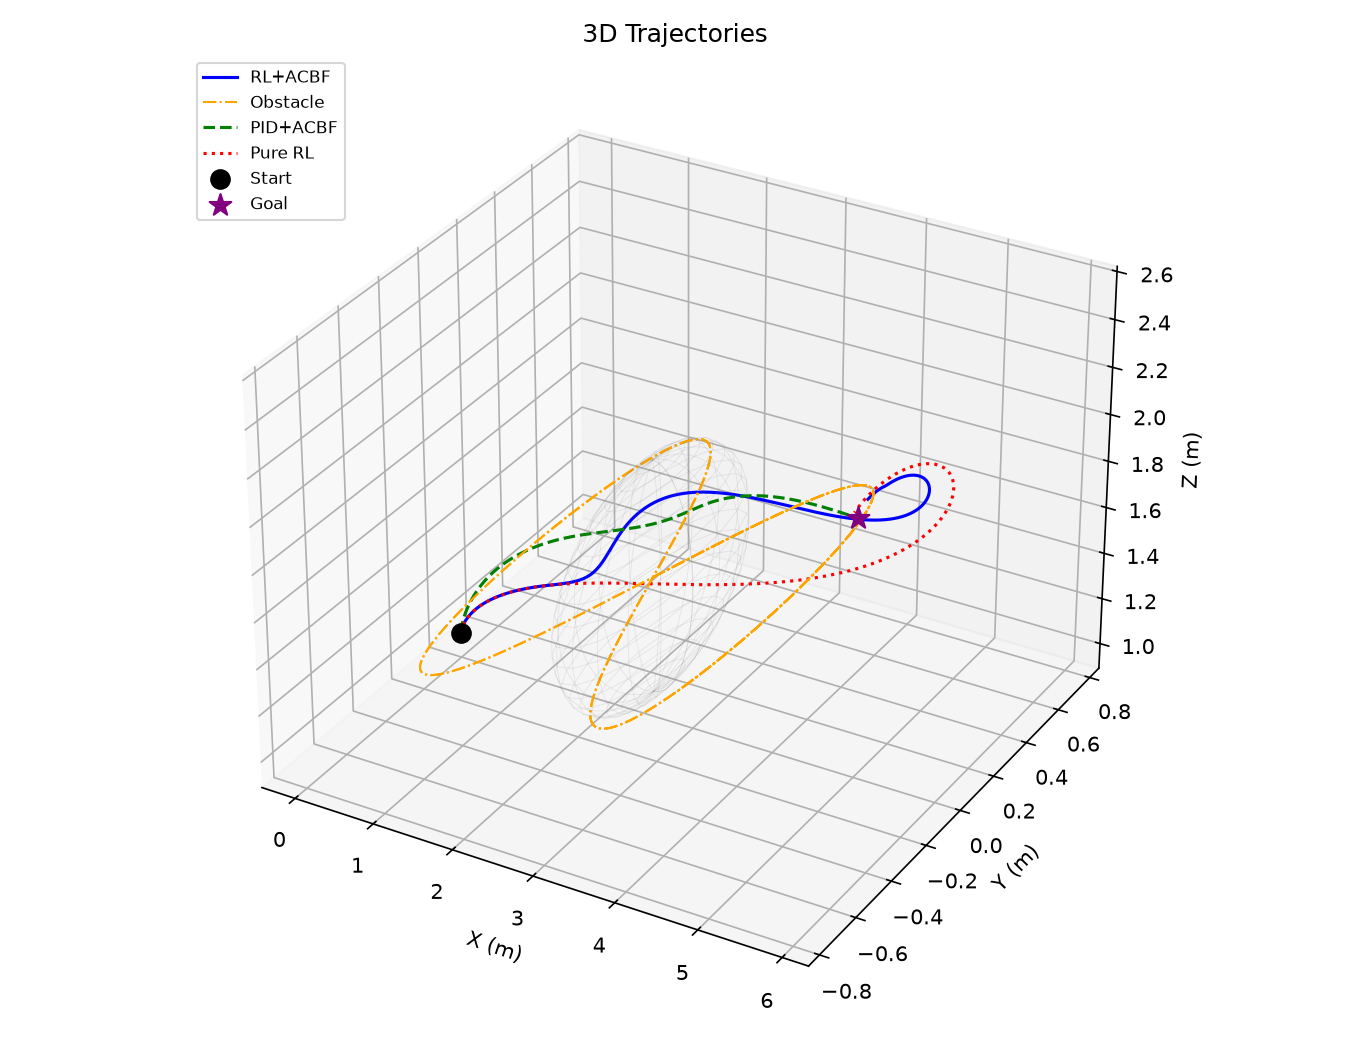
\includegraphics[width=.72\textwidth]{case3_trajectory.png}
\caption{Case 3 trajectories for the selected checkpoint. PPO+ACBF and PID+ACBF use the same obstacle predictor and filter but different nominal commands.}\label{fig:case3}
\end{figure}
\begin{figure}[htbp]\centering
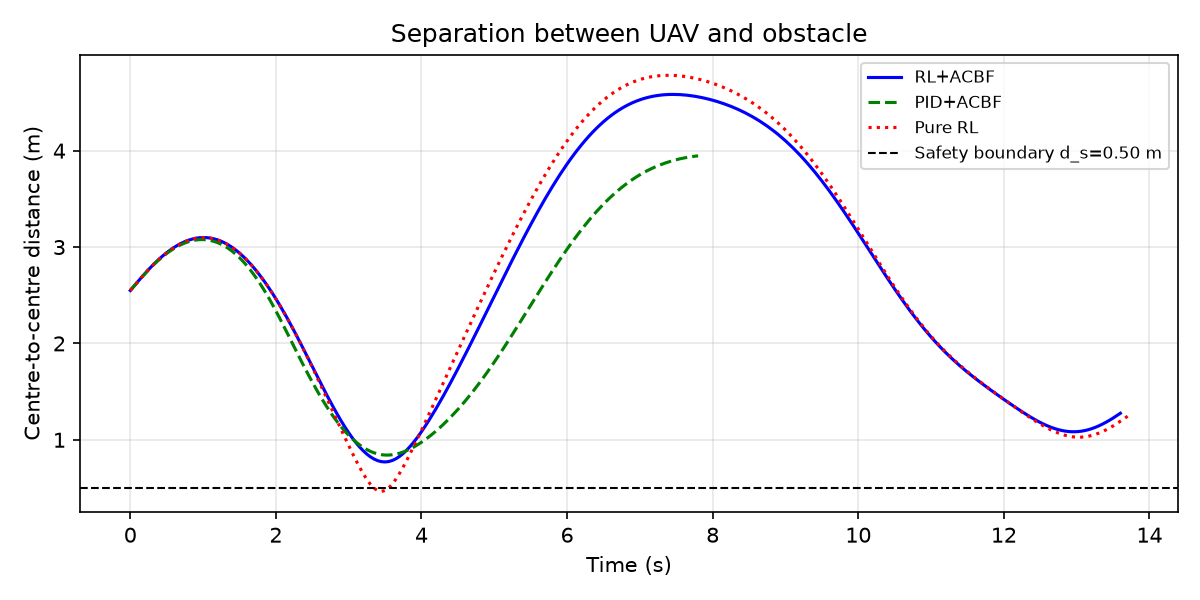
\includegraphics[width=.94\textwidth]{case3_separation.png}
\caption{Time-aligned centre separation in case 3. Pure RL enters the buffer; the filtered methods remain above it in these flights. Distance after a method's arrival is not evaluated because its episode has ended.}\label{fig:separation3}
\end{figure}

PID+ACBF reaches the goal in 7.80~s and maintains 0.842~m minimum separation. It therefore remains the stronger controller on both arrival time and minimum separation in this particular case. More generally, its mean scenario arrival time is 7.75~s, compared with 13.70~s for selected PPO+ACBF. The local results do not support a claim that RL is superior to PID on all evaluated metrics.
\FloatBarrier

\section{Final-checkpoint comparison}
Table~\ref{tab:final} reports the final 670,000-step checkpoint separately. It reaches the shared goal in every case, but its behavior differs from the selected checkpoint. Pure RL takes 17.10~s in each case and enters the figure-eight buffer. ACBF preserves the buffer and leads to earlier arrival in cases 2 and 3, at 12.15 and 12.70~s. The safety filter changes the entire subsequent closed-loop trajectory, so it can sometimes improve arrival time even though its objective is to stay close to the nominal command at each sample.

\begin{table}[htbp]\centering\small
\caption{Separate comparison using the final 670,000-step checkpoint. PID rows are repeated for consistent comparison and are not independent repeated trials.}\label{tab:final}
\begin{tabular}{llrrrr}
\toprule
Case & Controller & Time (s) & Error (m) & $d_{\min}$ (m) & Path (m)\\
\midrule
1 & Pure RL & 17.10 & 0.097 & 2.042 & 7.198 \\
1 & RL+ACBF & 17.10 & 0.097 & 2.042 & 7.198 \\
1 & PID+ACBF & 7.60 & 0.086 & 1.828 & 5.087 \\
\addlinespace
2 & Pure RL & 17.10 & 0.097 & 1.040 & 7.198 \\
2 & RL+ACBF & 12.15 & 0.096 & 1.186 & 6.799 \\
2 & PID+ACBF & 7.85 & 0.087 & 1.003 & 5.095 \\
\addlinespace
3 & Pure RL & 17.10 & 0.097 & 0.465 & 7.198 \\
3 & RL+ACBF & 12.70 & 0.085 & 0.749 & 6.853 \\
3 & PID+ACBF & 7.80 & 0.085 & 0.842 & 5.099 \\
\bottomrule
\end{tabular}
\end{table}

The final and selected models tie on additional goal success but differ in arrival times and the residual error of their shared failed goal. Retaining both provides a more complete picture than reporting whichever checkpoint is best for each metric. The results in the main trajectory figures all use the selected checkpoint.

\section{Diagnosis of earlier near-goal failures}
An earlier run's selected checkpoint at 340,000 transitions approached the scenario goal but stopped outside the tolerance. Pure RL finished approximately 0.424~m away after 25~s. Extending an obstacle-distant diagnostic flight to 60~s left it almost stationary 0.407~m away. A static policy probe found a zero-command position matching that endpoint closely. This identified a learned position bias, rather than merely insufficient episode duration.

Translated short-distance tests provided further evidence: the same 0.2~m relative movement succeeded near the fixed training start but failed near the distant scenario target. Since the observation contains absolute position, a policy can learn different local responses at different locations. The curriculum's early concentration around a fixed start is a plausible contributor. However, no controlled retraining ablation has established that removing absolute position alone would fix this behavior. The latest model substantially reduces the problem, but the remaining distant-goal timeout shows that precise positioning is not perfect everywhere.

\section{Computational and safety limitations}
For the selected PPO+ACBF checkpoint, recorded 95th-percentile control times are approximately 23.4, 116.2 and 118.8~ms in cases 1--3. The intended control interval is 50~ms. These timing measurements were collected during concurrent diagnostic work, so an isolated benchmark is required before drawing a hardware-speed conclusion. Nevertheless, the current measurements do not demonstrate real-time feasibility. Simulation arrival times must not be presented as wall-clock execution times.

The selected PPO+ACBF runs include one accepted inaccurate-solver step in case 2 and three in case 3. The implementation checks finite values and numerical residuals before accepting commands, but also permits higher-order slack. Successful geometry in these flights is an empirical result, not a proof that all barrier conditions hold exactly under every forecast error.

A previous checkpoint exposed a more serious limitation: in a figure-eight encounter, obstacle prediction overestimated next-step separation, the measured distance entered the safety buffer, and the following optimization was infeasible. The current policy avoids that failure in the tested trajectories, but no change to the predictor or filter has eliminated the underlying risk. Better navigation can reduce difficult encounters without making the safety layer universally robust.

\section{Threats to validity}
The results use a single training seed. The two reported checkpoints come from one run and must not be counted as independent learning repetitions. The additional goals are reused evaluation goals. The moving-obstacle cases share a start and destination, so three successful cases do not constitute three distinct destination-generalization tests. The environment uses prescribed obstacle motion and exact simulated position measurements, not a hardware perception stack.

There is no fixed-CBF baseline, no predictor ablation and no multiple-obstacle test. Therefore the study can attribute the paired difference to adding the complete IMM/ACBF layer for the same PPO policy, but cannot isolate how much of that difference comes from adaptation, the predictor, or other implementation choices. Collision counts are geometric, sampled metrics, and zero observed collisions in a finite set is not a universal probability statement.

\section{Discussion}
The evidence supports three conclusions. First, the implemented training procedure produces substantially improved navigation and satisfies its configured stopping condition. Second, the lower layer prevents the observed figure-eight buffer entry while retaining goal arrival for the evaluated policies. Third, the classical baseline remains faster and more direct. Together these results demonstrate a working hierarchical comparison with useful diagnostics, while defining clear boundaries on what can be claimed.

The most productive next step is broader validation rather than automatically increasing the training budget to its original ceiling. Independent seeds, varied start positions, new goal sets, prediction-error tests and isolated timing measurements would address the most consequential remaining uncertainties.
